\section{The Flatten-Then-Project Readout is Rank-Blind}
\label{sec:flat}

This section establishes the empirical phenomenon and its simplest
mechanism. \S\ref{sec:pc} shows that the mechanism is not the whole
story: readouts that escape it also produce flat curves.

\subsection{Four flat rank-$k$ curves}

We ran the matrix bottleneck under four training conditions that
vary the task, the CODI distillation weight $\gamma$, and the
multiplicative thinker. Each run produced a single rank-$k$ ablation
curve.

\begin{table}[t]
\centering
\small
\setlength{\tabcolsep}{3pt}
\begin{tabular}{llcclccc}
\toprule
Run & Task & $\gamma$ & Thinker & $\Z$ rank & k{=}1 & k{=}16 & $r_s$ \\
\midrule
R1 & GSM8K-Aug & 1.0 & on  & 5.5  & 6.00\% & 6.12\% & $-0.023$ \\
R2 & ProsQA    & 1.0 & on  & 10.2 & 78.4\% & 78.4\% & $+0.026$ \\
R3a & ProsQA   & 0.0 & on  & 12.7 & 76.8\% & 76.6\% & $-0.105$ \\
R3b & ProsQA   & 0.0 & off & 12.8 & 72.6\% & 72.4\% & $+0.095$ \\
\bottomrule
\end{tabular}
\caption{Rank-$k$ projection ablation across four training
conditions. $\Z$ rank is the mean effective rank of the $16\times16$
matrix thought at eval time. $r_s$ is the Spearman rank correlation
between per-sample effective rank and correctness. Range across
$k\in\{1,2,4,8,16\}$ is $\leq 0.6$pp in every row. Signs of $r_s$
are inconsistent across rows; $|r_s| < 0.11$ in all rows. Row R1
(GSM8K-Aug) is at a $6\%$ operating point where the model is below
any interpretable learning threshold; it is included for completeness
but does not constitute independent evidence.}
\label{tab:four-flat}
\end{table}

The result does not move when varying the task (arithmetic vs
logical reasoning), the distillation weight (removing the L1-at-colon
loss \emph{raises} effective rank from $\sim\!10$ to
$\sim\!13$, but does not change the curve shape), or the
multiplicative thinker (turning it off drops accuracy by
approximately one point but leaves the curve flat).
A negative control in \S\ref{sec:pc-negctrl} shows that this same
rank-$k$ probe applied to a vanilla GPT-2 SFT model --- one with no
$\Z$ at all --- also produces a flat curve and a random-$h$
sensitivity floor at the same accuracy. The flat curves in this section
are therefore necessary but not sufficient evidence on their own; the
model-level distinguisher is the three-seed decoupling result
(Fig.~\ref{fig:seed-decoupling}) below, which the negative control
cannot reproduce by construction.

\subsection{Why: the readout Jacobian is constant in $\Z$}

The flatten-then-project readout is $\phi(\Z) = W_{\text{down}}
\vecop(\Z)$. Its Jacobian with respect to $\Z$ is
\[
\frac{\partial\phi(\Z)}{\partial\Z_{ij}} \;=\; W_{\text{down}}[:,\,ij],
\]
which \emph{does not depend on $\Z$}. The loss gradient
$\partial\mathcal{L}/\partial\Z = (\partial\mathcal{L}/\partial\phi)\cdot
(\partial\phi/\partial\Z)$ is therefore a vector contracted with a
constant tensor. The contraction preserves the row-space of
$W_{\text{down}}$ but carries no information about the singular
structure of $\Z$.

\begin{proposition}[Constant-Jacobian rank-blindness]
\label{prop:jac}
Let $\phi:\R^{d\times d}\to\R^{D}$ be linear in $\Z$. Then for any
loss $\mathcal{L}$ differentiable at $\phi(\Z)$, the gradient
$\partial\mathcal{L}/\partial\Z$ is an affine function of
$\partial\mathcal{L}/\partial\phi$ alone, with coefficients
independent of $\Z$. The \emph{loss gradient through $\phi$} carries
no term that depends on the SVD basis of $\Z$. It follows that the
objective $\mathcal{L}$ itself provides no gradient signal preferring
one rank of $\Z$ over another. This is a local-gradient statement about
$\mathcal{L}$; implicit bias from the optimizer (Adam + weight decay)
and upstream parameter regularization may still shape the trained rank
through channels outside $\mathcal{L}$ (see \S\ref{sec:related} on
implicit low-rank bias).
\end{proposition}

\begin{proof}[Proof sketch]
If $\phi(\Z)=W\vecop(\Z)$ with constant $W$, then
$\partial\phi/\partial\Z_{ij}=W[:,ij]$ is a constant vector. By the
chain rule, $\partial\mathcal{L}/\partial\Z_{ij}$ is the inner
product of $W[:,ij]$ with $\partial\mathcal{L}/\partial\phi$, which
is independent of $\Z$'s SVD. Any invariance of $\mathcal{L}$ under a
change of $\Z$ that preserves the image $\phi(\Z)$ is therefore
preserved by gradient descent. \qedhere
\end{proof}

Proposition~\ref{prop:jac} is a direct consequence of the chain rule
applied to a linear map; it is not a deep theorem. Its value is
predictive: every linear-in-$\Z$ readout should produce a flat
rank-$k$ curve under pure loss-gradient training. The four training
conditions in Table~\ref{tab:four-flat} confirm this prediction;
\S\ref{sec:pc} tests what happens when the sufficient condition is
violated.

The same argument applies to any readout that factors through a
fixed-size linearly-derived space --- a linear low-rank factorization
of $W_{\text{down}}$, or a per-vocab bilinear logit head. All of these
have constant Jacobians and therefore produce rank-blind gradients
\emph{through the readout}.

\subsection{Accuracy is decoupled from rank across seeds}

Proposition~\ref{prop:jac} predicts that the loss landscape should
be flat along rank-changing directions of $\Z$: a model ending
training at rank $12$ and a model ending at rank $4$ can achieve the
same accuracy. We test this directly with three training seeds of
the same flatten-readout configuration (gpt2-small, ProsQA,
$\gamma=0$, 25 epochs, batch 16).

\begin{figure}[t]
\centering

\includegraphics[width=\linewidth]{figures/fig2_seed_decoupling.pdf}
\caption{Three-seed replication of the flatten readout. Best ProsQA
accuracy is tight at $81.51\pm 1.2$pp, but the final effective rank
of $\Z$ varies $3\times$ (seed 42 converges at rank $\sim\!4$; seeds
1337 and 7 converge near rank $12$). The loss does not push $\Z$
toward any particular rank.}
\label{fig:seed-decoupling}
\end{figure}

Figure~\ref{fig:seed-decoupling} directly demonstrates that the
matrix-bottleneck training objective does not reward rank: three models
at identical hyperparameters achieve statistically indistinguishable
accuracy at effective ranks spanning a $3\times$ range. The result is
not an ablation artifact: the accuracies are computed on the same test
split under standard decoding.

\subsection{Linear probe on $\Z$}

If rank is decoration, what \emph{does} $\Z$ carry? We ran a 5-fold
cross-validated multi-class logistic regression to predict the
ProsQA target class from a flattened $\Z$ on $500$ held-out test
problems. Controls: the same prompt's hidden state from a pretrained
GPT-2 with no ProsQA fine-tuning, and the same model at random
initialization.

\begin{figure}[t]
\centering
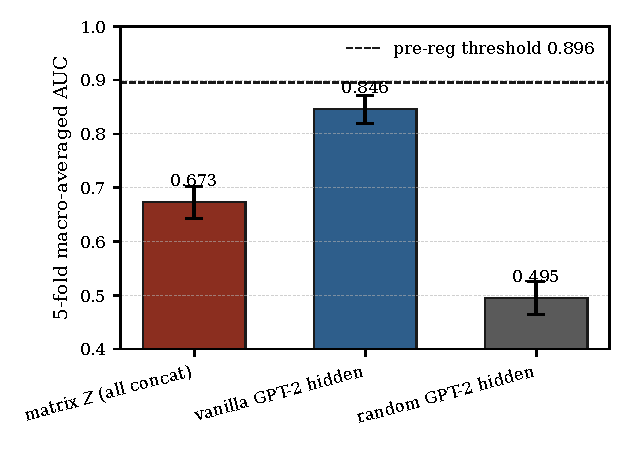
\includegraphics[width=\linewidth]{figures/fig5_linear_probe.pdf}
\caption{Linear probe AUC for ProsQA target class prediction.
Pre-registered threshold for a positive result was
$\max(\text{vanilla},\text{random})+0.05=0.896$. The matrix $\Z$
concat AUC of $0.673$ does not exceed it. Vanilla GPT-2 --- never
trained on ProsQA --- predicts the target class better than the
trained matrix-CODI bottleneck.}
\label{fig:probe}
\end{figure}

Vanilla pretrained GPT-2 reaches AUC $0.846$ at 768 features. The
matrix-CODI bottleneck's concatenated matrix thought (6 latent
positions $\times$ 256 features $= 1536$ features) reaches AUC
$0.673$ --- \emph{more} features than the vanilla hidden state,
\emph{lower} predictive signal for the ProsQA target. A
dimension-matched comparison (a probe on the post-bottleneck
reconstructed 768-dim hidden state $W_{\text{down}}\vecop(\Z)$ that
the downstream transformer consumes) is deferred to
camera-ready; the current data establish that the matrix bottleneck
does not recover target-predictive information commensurate with its
feature count. A binary target-vs-distractor probe on the same $\Z$
tensors is at chance (AUC $0.50$--$0.56$) across all conditions.

In combination, the flat rank-$k$ curves, the three-seed decoupling,
and the linear probe gap point to the same conclusion: the matrix
thought in a flatten-readout matrix-CODI does not construct reasoning
state. The structural capacity of $\Z$ is available but not used.
